% The format is not taking the image on the specific place. Look at the next 2 lines later
\documentclass[conference]{IEEEtran}
%\documentclass[journal,12pt, singlecolumn]{IEEEtran}

\pagestyle{plain}

\usepackage{lineno}
\usepackage[draft]{hyperref}
\usepackage{cite}
\usepackage{amsmath}
\usepackage{graphicx}
\usepackage{epstopdf}
\usepackage{enumerate}
\usepackage{filecontents}
\usepackage{epsfig}

\usepackage{float}
\usepackage{caption}
\usepackage{subcaption}
\usepackage{amssymb}
\usepackage{algcompatible}
\usepackage[linesnumbered,ruled]{algorithm2e}
\IEEEoverridecommandlockouts
\newtheorem{theorem}{Theorem}[section]
\newtheorem{lemma}[theorem]{Lemma}
\newtheorem{proposition}[theorem]{Proposition}
\newtheorem{corollary}[theorem]{Corollary}

\newcommand\norm[1]{\left\lVert#1\right\rVert}
\renewcommand\thetheorem{\arabic{section}.\arabic{theorem}}
\usepackage[usenames,dvipsnames]{color}
\newcommand{\dt}[1]{\textcolor{red}{{#1}}}
\newcommand{\sh}[1]{\textcolor{blue}{{#1}}}

\newcommand{\spl}[1]{\mathcal{#1}}
%%%%%%%%%%%%%%%%%%%%%%%
\begin{document}

\title{Non-Intrusive Deployment of Blockchain in Establishing Cyber-Infrastructure for Smart City\thanks{978-1-7281-2294-6/19/\$31.00 \text{\textcopyright}2019 IEEE}}
% 

\author{\IEEEauthorblockN{Adeel A. Malik$^1$, Deepak K. Tosh$^1$, Uttam Ghosh$^2$}
	\IEEEauthorblockA{
		$^1$Department of Computer Science, University of Texas at El Paso, TX, USA \\
		$^2$Department of Computer Science, Vanderbilt University, USA \\
	    amalik@miners.utep.edu, dktosh@utep.edu, uttam.ghosh@vanderbilt.edu
	}
}

\maketitle

\begin{abstract} 
Internet-of-Things has emerged to develop smart communities so that real time sensing and decision can improve operational efficiency and quality of lives. However, establishing such infrastructure can be exceptionally intricate due to the vast variety of devices and the implemented technologies. Also, it poses several unique challenges, such as heterogeneity of the infrastructure, type, and scale of deployment, security, privacy, and inter-operability. One primary concern in a smart city environment is the capabilities of typically end-IoT devices which are vulnerable to security threats and prone to confidentiality and integrity breach of data. Blockchain can potentially address these security challenges due to the distributed ledger's inherent properties. In this paper, we propose a decentralized architecture using the Blockchain to provide a secure and resilient smart city infrastructure that can run the ledger service over a distributed network. We consider a permissioned Blockchain, Hyperledger Sawtooth, and to automate and to overcome the infrastructural challenges concerning the smart city deployment, and we provide a systematic methodology that automates the deployment process and saves a significant amount of time. We simulate and deploy a Blockchain-integrated smart city environment using the proposed seamless deployment strategy using our automation module. With the proposed deployment scheme, we improve the Blockchain-based infrastructure development time by 82\% compared to the traditional deployment approach.
\end{abstract}

\begin{IEEEkeywords}
Blockchain, Smart City, Hyperledger Sawtooth, Decentralized Deployment. 
\end{IEEEkeywords}

\section{Introduction}
\label{sec:introduction}
%\vspace{0.10in}
Internet-of-Things (IoT) \cite{dorri_Blockchain_2017} devices are influencing our daily lives in many ways by collecting and sharing data from the operating environment with the help of attached sensors. IoTs are gaining popularity and are widely used nowadays in smart home applications, medical and healthcare, transportation, manufacturing, supply chain \cite{liangEDS}, battlefield \cite{toshIOBT} and electric grids. In the case of a smart home, many connected devices receive/transmit data among themselves and to the outside world. The same example when expanded on a broader scale, a ``smart city''\cite{chourabi_understanding_2012}, where many different types of devices and technologies are integrated to monitor city operations will generate a vast amount of data. Thus the security and trustworthiness of each data point are critical for achieving efficiency in smart city applications. The concept of a smart city is still emerging, and some of the applications include smart parking, traffic congestion, smart grids \cite{ghoshsmartgrid2016}\cite{ghosh2017security}\cite{ghosh2019security}, etc. 

With the advancements of IoT and cyber technologies, the cities can be transformed to establish a connected, inter-operable, and highly automated infrastructure that will assist in taking effective decisions in real-time while achieving the necessary safety and security requirements of the society. However, instantiating such a huge cyber-infrastructure for the smart city applications can be overwhelming unless a systematic and well-analyzed deployment strategy is in place. There can be several unique challenges while deploying the infrastructure in a seamless manner, which can be categorized as follows:
(1) nature of the Infrastructure (complicated, costly, and technologically challenged);
(2) type of deployment (centralized, decentralized, distributed);
(3) scale of deployment (deployment, powering, and data collection from the devices);
(4) security of the infrastructure (authentication, validation, and access protection); 
(5) privacy (data confidentiality);
(6) inter-operability (interfacing heterogeneous systems).

Furthermore, the IoT devices usually are not computationally robust devices, and typically have limited processing power to execute core application functionalities. At the same time, there can be millions of sensors and other connections in a centralized fashion which introduces additional overhead in achieving data security and resiliency while communicating with the cloud server. Authors in  \cite{alaba_internet_2017} present an extensive study and a taxonomy on IoT security threats and vulnerabilities. The study discusses an IoT security scenario and proposes a client-server model. However, the proposed security model is not able to achieve the ideal secured environment due to the limitations of the IoT environment. Blockchain \cite{toshsecurity2017}, on the other hand, it provides a secure decentralized framework that eliminates single points of failure and offers critical security and resilient properties through its tamper-resistant distributed ledger. To achieve secure and resilient cyberinfrastructure in a smart city, the Blockchain technology can be considered as a potential candidate since the critical element of Blockchain, and the reason for its tremendous potential is the unchanging nature of its blocks. Blockchain offers the likelihood to have all the data in a single database with members having predefined authorizations to view or change the data they need. However, the difficulty involved in deploying Blockchain nodes one at a time requires an automated technique to build the infrastructure in a non-intrusive way.

In this paper, our contributions are the following: 1) propose a decentralized architecture for a smart city cyber infrastructure, 2) provide a non-intrusive Blockchain infrastructure implementation strategy to accommodate distributed nature and security needs of IoT-enabled smart city. Since it is essential to automate the bootstrapping process without redundant work in setting up a smart city infrastructure, we investigate the issue of automating the bootstrap process for Blockchain peers in a high node dynamism environment. To realize this scenario, we implement a simulated smart city environment (Fig. \ref{fig:Main_Architecture}) where different edge servers mimic the role of city departments that are deployed to collect and process data from connected devices and distribute them across other departments. Using a permissioned Blockchain, Hyperledger Sawtooth \cite{hyperledger-sawtooth}, and our proposed automation module, we demonstrate the seamless deployment of Blockchain infrastructure for the smart city use case. The proposed automation methodology results 82\% of deployment efficiency compared to traditional Blockchain deployment, thus significantly reduces the sequential deployment overheads.

The paper is organized as follows. In Section \ref{sec:Background}, we highlight the background and related work. Section \ref{sec:Architecture} discusses the proposed architecture and different deployment scenarios. In section \ref{sec:Evaluation}, we evaluate the results and discuss the observations. Section \ref{sec:Conclusion} discusses the findings and future directions. 



\section{Background}
\label{sec:Background}
%\vspace{0.10in}
% Use PNG or PDF file formats and no spaces
IoTs offer a promising future, and the idea of smart cities has grown impressively with the ascent and improvement of the IoT advancement. Smart cities are distributed systems that enable a diverse set of services over multiple layers of communication. Due to these characteristics a general architecture to fit all sizes is challenging. Andrea Zanella et al. \cite{zanella_internet_2014} present a framework that targets smart city street light application to collect environmental data (e.g. CO level, temperature, humidity, etc.) through wireless nodes placed on street lights to ensure the correct operation of the public lighting system. The study results demonstrate that the current technologies have achieved the dimension of development to permit the pragmatic acknowledgment of IoT solutions. 

In another study, Yibin Li et al. \cite{li_privacy_2016} address the privacy concern by presenting a mobile-cloud framework to protect user-data from smartphones and a proof-of-concept for the proposed benchmark to prevent data over-collection. The study shows the level of security risks in non-iOS devices is more frequent then iOS devices due to the locked development environment for iOS applications. The study also identifies the permission model of current mobile phones which is limited to allow full permission or none. The proposed benchmark overcomes this limitation and provides a customized permission model to address the data over-collection problem. P.G.V Naranjo et al. \cite{naranjo_focan:_2018} propose FOCAN, a Fog-supported multi-tire smart city network architecture that supports communications between heterogeneous systems through a smart city environment. The study supports Fog computing and aims to focus on scalability, energy saving, and low latency by introducing additional Fog layer in a distributed smart city environment. 

SpeedyChain is a new Blockchain-based framework~\cite{michelin_speedychain:_2018} that provides a private and secure communication model for smart vehicles. It also ensures data integrity using hashes in transactions as well as the communication auditability using transaction records in the Blockchain. The proposed framework decouples the block header and the transaction data to enable faster data addition to the block. The experiment results show a linear growth in time, showing low latency introduced by the proposed framework and the possibility to exchange information in smart cities ensuring resilience, data integrity and tamper-resistance.

On one hand, it is essential to understand the strengths and weaknesses of the Blockchain technology before implementation. Authors in \cite{dinh_untangling_2018} conducted a comprehensive study between three different Blockchain applications (Ethereum, Parity and Hyperledger) in terms of their data processing capabilities with the help of a proposed benchmark called ``BLOCKBENCH". The benchmark narrows the design space to get focused insights on the design trade-offs and performance bottlenecks. On the other hand, it is equally important to understand the concept of smart cities. Hafedh Chourabi et al. \cite{chourabi_understanding_2012} proposed a framework to understand smart cities where they have identified critical factors of smart city initiatives. Authors in \cite{liangsmartcity} analyze potential security concerns while integrating Blockchain in smart city infrastructure for enahnced resilience.

In all of the related studies, none of the researchers have emphasized the actual node deployment for a smart city infrastructure. This paper aims to provide adaptability in characterizing and deploying the smart city node framework, empowering a city IT administrator to customize the network size with any number of nodes. In the next section, we will discuss the deployment methodology for an experimental smart city architecture with different deployment scenarios.  

\section{Distributed Architecture for Smart City}
\label{sec:Architecture}
%\vspace{0.10in}
Smart cities offer improved infrastructure for various public sector applications utilizing different technologies and devices. In a typical smart city environment, there are coherent data communications between heterogeneous entities and systems. To make better decisions, data integrity is vital along with security and confidentiality. To realize this scenario, in this section, we deploy Blockchain-based nodes in a smart city environment, Fig. \ref{fig:Main_Architecture} explains the architecture where different city departments (City HQ, Traffic and Police, Communications, Education and Healthcare) have several subsystems and IoTs that share data with their representative central servers. Each of these representative servers is a peer on the Blockchain network and responsible for sharing with other peers (Fig. \ref{fig:Sawtooth_Architecture}). To simplify the deployment process, we propose a methodology and simulate the smart city nodes and the network.

\begin{figure}[!ht] % H for place here
    \centering
    \setlength{\belowcaptionskip}{-10pt}
    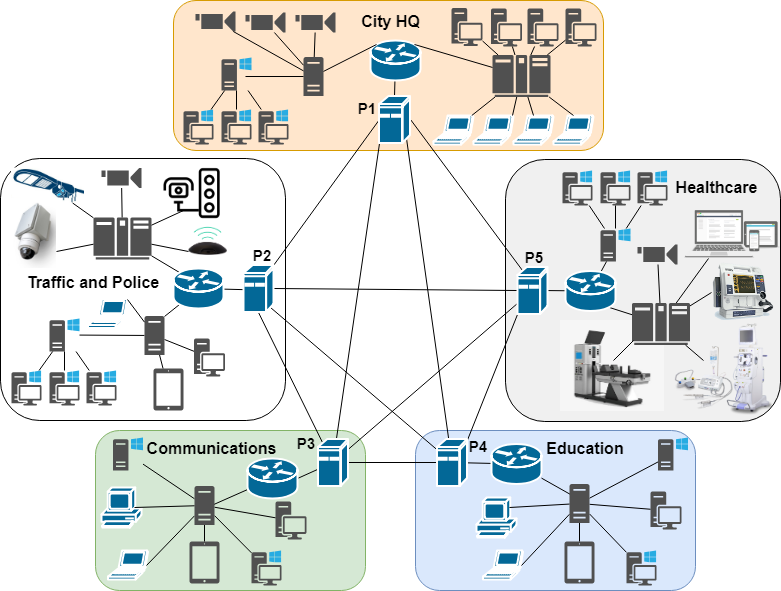
\includegraphics[scale=.30]{figs/main_arch.png}
    \caption{Smart City Environment Architecture}
    \label{fig:Main_Architecture} %refer the figure with this label
\end{figure}

\begin{figure*}[!ht] % ! force and t next page top
    \centering
    \setlength{\belowcaptionskip}{-10pt}
    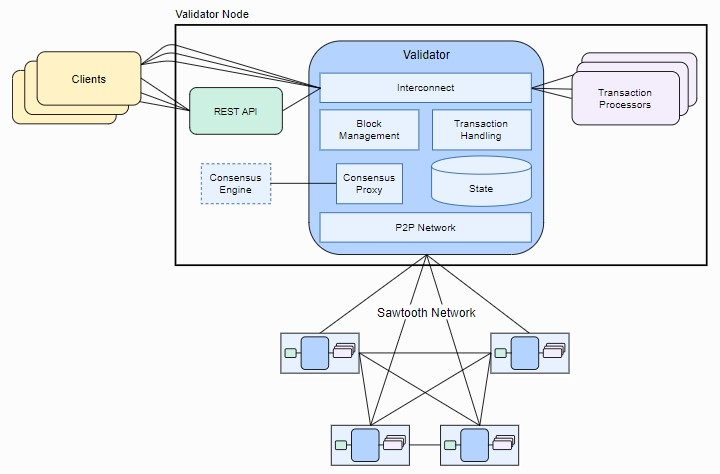
\includegraphics[width=5in]{figs/sawtooth_arch.png}
    \caption{Sawtooth Architecture \cite{sawtooth-architecture-guide}}
    \label{fig:Sawtooth_Architecture} %refer the figure with this label
\end{figure*}

\subsection{Methodology}
The nodes are deployed in the following fashion:

\textbf{(1) Genesis Node Deployment}: The first node on the Blockchain network contains the genesis block. Genesis block is the first block and the root of the Blockchain. This block does not contain any transactions. However, it contains the configuration settings which are used to bootstrap the very first validator node. The genesis block is then forwarded to the other peer nodes upon joining to the Blockchain network. Deployment and configuration of genesis node is a necessary prerequisite for allowing other validator nodes to join the Blockchain infrastructure.

\textbf{(2) Validator Nodes Deployment}: Any node joining the Blockchain network after the genesis node will initially connect to either the genesis node or any other fully functional peer in the Blockchain network to obtain the necessary information and settings about the genesis block. This deployment phase can run in parallel or sequentially. In each case, the genesis node has to be deployed first, and the rest of the validator nodes can be deployed sequentially or in parallel afterwards. Table I explains the total time taken by sequential and parallel deployments.

\begin{table}[H]
\centering
\label{tab:dep_times}
\begin{tabular}{|l|l|}
\hline
Deployment Type & Deployment Time   \\ \hline
Sequential      & 37min 53sec.      \\ \hline
Parallel        & 6min 42sec.       \\ \hline
\end{tabular}
\caption{Total deployment overheads.}
\vspace{-4mm}
\end{table}

To automate the deployment, we have created a deployment script\footnote{https://goo.gl/ic3Z1F} that allows a city IT administrator to deploy any number of validator nodes to establish the decentralized P2P network for running the ledger service easily. The script execution enables the user to select between deployment (Genesis/Validator node) and peering modes (Static/Dynamic). Fig. \ref{fig:script} explains the overall flow of the script functionality which is mainly divided into three main phases as highlighted in different colors. The phases are explained as below:

\begin{figure}[H] % H for place here
    \centering
    \setlength{\belowcaptionskip}{-10pt}
    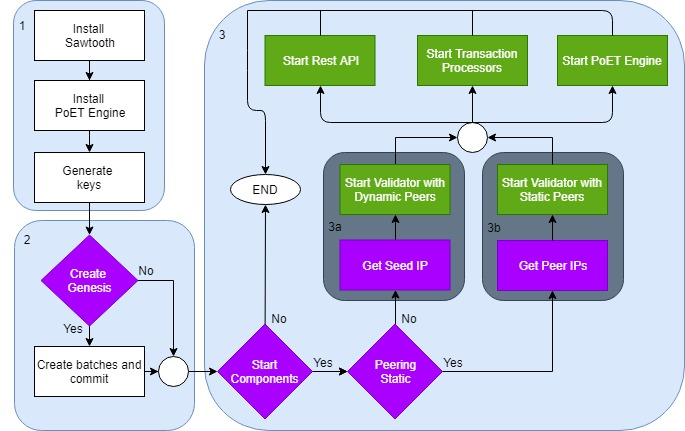
\includegraphics[scale=.60]{figs/block_diagram.png}
    \caption{Block diagram of the automation script}
    \label{fig:script} %refer the figure with this label
\end{figure}

\textbf{Phase 1: Sawtooth Deployment}: This phase runs on each node by default whenever the script is executed and deploys the required Sawtooth components.

\textbf{Phase 2: Genesis Block Creation}: This is an optional phase to deploy the genesis block with the chain configuration settings required for bootstraping validator nodes. In case of the first node, the user will pass ``Y'' as the first parameter to deploy the genesis block on the first node and ``N'' for the validator nodes to skip this phase.

\textbf{Phase 3: Starting Components}: This phase starts the Sawtooth components (Fig. \ref{fig:script} green boxes) that are required in order to bring the node up on the Sawtooth network. This phase is also optional, and the user can decide to run or skip this phase. In the case, if the user chooses to skip this phase, there is an additional script provided just for this phase to start the components. The additional script ``start\_components\_poet.sh'' instead of running the entire deployment process from the beginning, starts the components and takes peering options as parameters. The area highlighted grey (3a and 3b) in the Fig. \ref{fig:script} phase 3, is the peer/seed selection options (Dynamic or Static \cite{sawtooth-peering}) that allows the user to customize based on how the user wants the current node to peer up with the existing network. With dynamic peering, the new nodes can join without having to restart existing node's components or specifying IP addresses of existing nodes and in case of static peering, only pre-defined peers that can connect. For this phase, the user needs to pass three parameters (Param 2, 3 and 4 Table II).

\subsection{Deployment Categories}
This section discusses different deployment scenarios that we can have while simulating the Blockchain-based smart city infrastructure. Each scenario is explained further using a table containing user parameters that needs to be passed while initiating the deployment process. Fig. \ref{fig:peering} refers to the overall deployment of nodes.

\begin{figure}[H] % H for place here
    \centering
    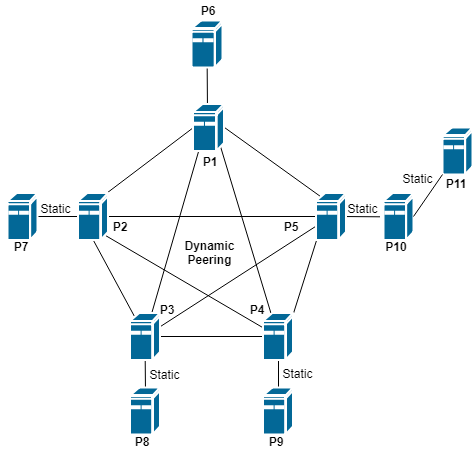
\includegraphics[scale=.5]{figs/peering.png}
    \setlength{\belowcaptionskip}{-5pt}
    \caption{Full network topology (Dynamic and Static peering)}
    \label{fig:peering} %refer the figure with this label
\end{figure}

\textbf{Scenario 1: First node (Genesis) deployment}: 
In this case, the user is trying to deploy the first node for the Blockchain network that will contain the genesis block. For this case, we assume that the user wants to start the components with the “Dynamic” peering mode. This scenario well suites for node ``P1'' (Fig. \ref{fig:peering}) under the City HQ department in the smart city simulation. 

For this scenario, the following parameters will be passed:
\begin{table}[H]
\centering
\label{tab:genesis_install}
\begin{tabular}{|l|l|}
\hline
Parameter 1: Create Genesis block? & Y         \\ \hline
Parameter 2: Start components      & Y         \\ \hline
Parameter 3: Peering static?       & N         \\ \hline
Parameter 4: Seed IP:              & tcp://current-machine-IP:port \\ \hline
\end{tabular}
\caption{Genesis node deployment.}
\vspace{-4mm}
\end{table}

Since this is the first node on the network, the seed IP will be the IP address of the current node. 

\textbf{Scenario 2: Validator node deployment (Known Genesis)}: 
In this case, the user is trying to deploy a peer node after the genesis node is up and running. The genesis node should be running with Dynamic peering mode actively looking for peers to connect. 
For this node, we are assuming that the user is aware of the IP address of the genesis node and wants to run the components under the ``Dynamic'' peering mode. This case can be applied to each departmental servers (Fig. \ref{fig:Main_Architecture} P2-P5).

For this scenario, the following parameters will be passed:
\begin{table}[H]
\centering
\label{tab:node_n_install}
\begin{tabular}{|l|l|}
\hline
Parameter 1: Create Genesis block? & N                          \\ \hline
Parameter 2: Start components      & Y                          \\ \hline
Parameter 3: Peering static?       & N                          \\ \hline
Parameter 4: Seed IP:              & tcp://genesis-node-ip:port \\ \hline
\end{tabular}
\caption{Validator node deployment - Known Genesis.}
\vspace{-4mm}
\end{table}
Since this is not the first node on the network, we will not create the genesis block on this node but provide the IP address of the seed, i.e. either the genesis node or any active peer that has already become a peer with the genesis node.

\textbf{Scenario 3 – Validator node deployment (Unknown Genesis)}: 
In this case, the user is trying to deploy a peer node after the genesis node is up and running and the user is not aware of the genesis node’s IP address. However, the IP address another active peer is known. As we see in Fig. \ref{fig:peering}, P10 is connected with P5 and similarly P11 with P10. For this case, we are assuming that these nodes are connecting with their neighbors under ``Dynamic'' peering mode. This scenario can apply to any node on the network which is not connected directly with the genesis node. 

For this scenario, the following parameters will be passed:
\begin{table}[H]
\centering
\label{tab:node_n_install2}
\begin{tabular}{|l|l|}
\hline
Parameter 1: Create Genesis block? & N                          \\ \hline
Parameter 2: Start components      & Y                          \\ \hline
Parameter 3: Peering static?       & N                          \\ \hline
Parameter 4: Provide seed(s) IP:   & tcp://seed-node-ip:port    \\ \hline
\end{tabular}
\caption{Validator node deployment - Unknown Genesis.}
\vspace{-4mm}
\end{table}

\textbf{Scenario 4 – Validator node deployment (Static peering)}: 
For this scenario, we are assuming the user wants to deploy a peer node with predefined fixed peers instead of dynamic. 

For this scenario, the following parameters will be passed:
\begin{table}[H]
\centering
\label{tab:node_n_install2}
\begin{tabular}{|l|l|}
\hline
Parameter 1: Create Genesis block? & N                          \\ \hline
Parameter 2: Start components      & Y                          \\ \hline
Parameter 3: Peering static?       & Y                          \\ \hline
Parameter 4: Provide peer(s) IP:   & tcp://peering-node-ip:port \\ \hline
\end{tabular}
\caption{Static node deployment.}
\vspace{-4mm}
\end{table}

For ``Static'' peering, port numbers are also required. If there are more than one static peers, they can be specified with a comma, e.g.: ``tcp://peering-node1-IP:port\#,tcp://peering-node2-IP:port\#,...''

\textbf{Test Scenario 5 – Churning validator node deployment}: 
Any node on the network can go down at any point. In this case, an existing peer, e.g. P3 (Fig. \ref{fig:peering}) from the Blockchain network goes offline for some period and comes back online. We are assuming that the user will start the components under dynamic peering mode in this case.

For this scenario, the following parameters will be passed:
\begin{table}[H]
\centering
\label{tab:node_n_install2}
\begin{tabular}{|l|l|}
\hline
Parameter 1: Create Genesis block? & N                          \\ \hline
Parameter 2: Start components      & Y                          \\ \hline
Parameter 3: Peering static?       & N                          \\ \hline
Parameter 4: Provide peer(s) IP:   & tcp://active-peer-ip:port  \\ \hline
\end{tabular}
\caption{Churning node deployment.}
\vspace{-4mm}
\end{table}

In Fig. \ref{fig:peering}, it is seen that node P3 is acting as a peer node for P8 as well, and the downtime for P3 isolates the P8 node from the Blockchain network. Similarly downtime for P5 isolates P10 and P11 from the entire network. In the next section, we will discuss and evaluate all of the above scenarios to find out the outcome. 

\section{Performance Evaluation}
\label{sec:Evaluation}
%\vspace{0.10in}
In order to evaluate our proposed automated deployment strategy, we start with the initial Sawtooth network with five nodes. All nodes on the Sawtooth network will include the basic Sawtooth components as shown in Fig. \ref{fig:Sawtooth_Architecture}), a Validator, REST API and set of Transaction Processors running. The first node creates and distributes the genesis block. For simplicity, the authorization type between the nodes is set to default ``trust'' option, where nodes can communicate to each other without additional authentication setup. Each node is allocated the following specifications: \textbf{Memory}: 2GB, \textbf{Processor}: 2 CPUs, \textbf{Storage}: 20GB, \textbf{Network}: NAT, \textbf{OS}: Ubuntu 16.04 LTS. To simulate the nodes and network, we are using Oracle's VirtualBox\cite{oracle-virtualbox}. 

To evaluate the scenarios described in the previous section, we have designed the following network topology (Fig. \ref{fig:peering}) with 11 nodes, where five nodes (P1-P5) connect via dynamic peering and six nodes (P6-P11) connect via static peering.

The following table describes the node details, selected peering option and the time taken by the deployment script to bring the node up in order to successfully join the Blockchain network. Once the genesis node is up and running, the remaining nodes can be deployed in parallel in the case of dynamic peering, and sequential in case of static peering. The following table contains the results from a sequential deployment. 

\begin{table}[h]
\centering
\label{tab:node_details_dep}
\begin{tabular}{|l|l|l|l|l|}
\hline
Node       & IP        & Peering & Peer/Seed & Deployment Time \\ \hline
P1-Genesis & 10.0.1.10 & Dynamic & 10.0.1.10 & 2min 42sec.  \\ \hline
P2         & 10.0.1.11 & Dynamic & 10.0.1.10 & 2min 50sec.  \\ \hline
P3         & 10.0.1.12 & Dynamic & 10.0.1.10 & 3min         \\ \hline
P4         & 10.0.1.13 & Dynamic & 10.0.1.10 & 2min 35sec.  \\ \hline
P5         & 10.0.1.14 & Dynamic & 10.0.1.10 & 2min 57sec.  \\ \hline
P6         & 10.0.1.15 & Static  & 10.0.1.10 & 3min 05sec.  \\ \hline
P7         & 10.0.1.16 & Static  & 10.0.1.11 & 3min 10sec.  \\ \hline
P8         & 10.0.1.17 & Static  & 10.0.1.12 & 2min 44sec.  \\ \hline
P9         & 10.0.1.18 & Static  & 10.0.1.13 & 2min 59sec.  \\ \hline
P10        & 10.0.1.19 & Static  & 10.0.1.14 & 3min 15sec.  \\ \hline
P11        & 10.0.1.20 & Static  & 10.0.1.19 & 3min 20sec.  \\ \hline
\end{tabular}
\caption{Node details and deployment time.}
\vspace{-4mm}
\end{table}

The total time taken in case of a sequential deployment is 32 minutes and 37 seconds and the average time taken by each node is 2 minutes and 57 seconds. Moreover, the deployment time mainly depends on two more factors, the node’s processing capabilities (as described in the architecture section) and the available internet speed, which in our case on an average at the time of experiment was 85 Mbps down and 85 Mbps up.

In case of known and unknown genesis, regardless of static or dynamic peering modes selected, once all nodes are up and running, the latest transactions from each of the nodes are synchronized on all other peers of the Blockchain network. We are experimenting with a few basic transactions on different nodes and verifying the same on all other nodes. Since the transactions are very small, they are reflected immediately.

\begin{figure}[H] % H for place here
    \centering
    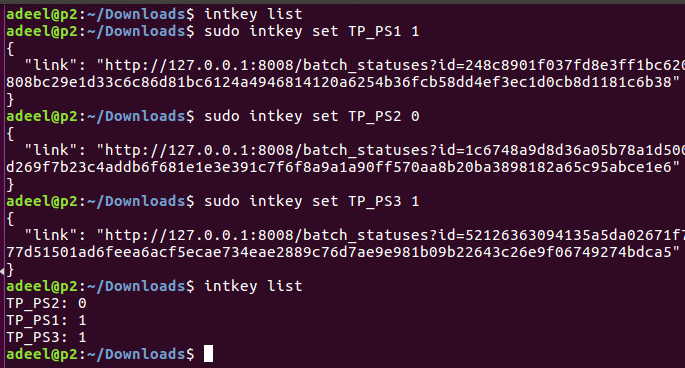
\includegraphics[scale=.60]{figs/1TP_Trans.PNG}
    \setlength{\belowcaptionskip}{-15pt}
    \caption{Transactions (Parking Sensors Data) from Traffic and Police Department on P2}
    \label{fig:p1} %refer the figure with this label
\end{figure}

\begin{figure}[H] % H for place here
    \centering
    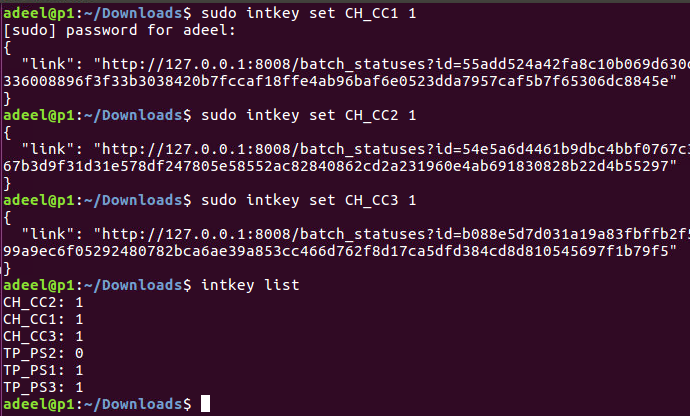
\includegraphics[scale=.60]{figs/2CQ_Trans.PNG}
    \setlength{\belowcaptionskip}{-15pt}
    \caption{Transactions (City HQ CCTV Data) from City HQ on P1}
    \label{fig:p2} %refer the figure with this label
\end{figure}

We use intkey command to create sample IntegerKey transactions. As seen in Fig. \ref{fig:p1}, the initial intkey list command returns no values. However, as we start making transactions on each client, the intkey list command starts returning newly added values. Fig. \ref{fig:p3} shows the entire intkey list synchronized on the last node.

\begin{figure}[H] % H for place here
    \centering
    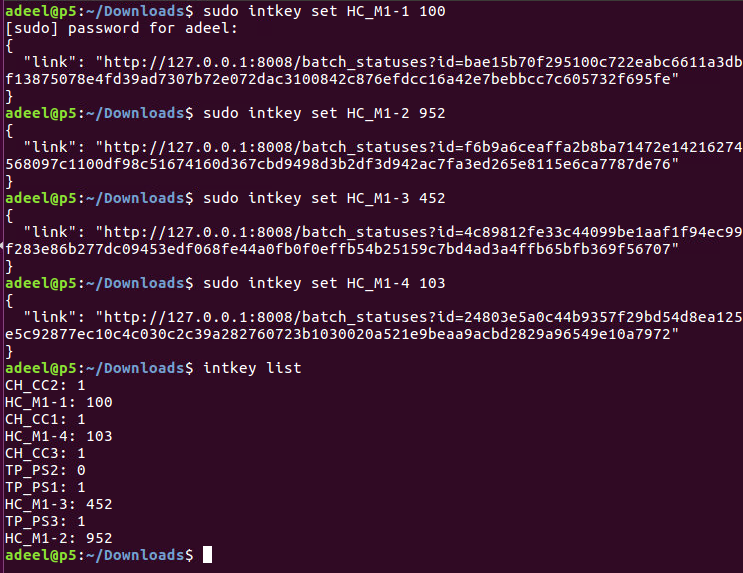
\includegraphics[scale=.50]{figs/3HC_Trans.PNG}
    \setlength{\belowcaptionskip}{-15pt}
    \caption{Transactions (Healthcare Data) from Healthcare on P5}
    \label{fig:p2} %refer the figure with this label
\end{figure}

\begin{figure}[H] % H for place here
    \centering
    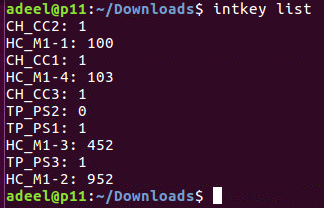
\includegraphics[scale=0.8]{figs/4P11_Trans.PNG}
    \setlength{\belowcaptionskip}{-5pt}
    \caption{Synchronized transactions from all nodes on P11}
    \label{fig:p3} %refer the figure with this label
\end{figure}

In case of the “Churning Node”, we turn off node P10 for some time. Node P10 bridges P13 with the rest of the Blockchain network. A few transactions are made during this time on the other nodes (P1-P9) and a few transactions on the isolated node P11. Peering between P11 - P10 and P10 - P5 is ``Static''. It is observed in this case that P11 is not able to transfer any transactions to the chain. While the only peer of P11 is offline and there is no other peer to agree on the transactions made by P11, those transactions are ignored and not synchronized on the chain. In the case of dynamic peering, there has to be at least one more peer actively running apart from the peer making the transaction to add the transactions to the chain. After P10 comes back online, it fetches the latest updates from its peer P5. However, P11's components need to be restarted for P11 to fetch the latest updates from P10. 

If P5 is down, isolating P10 and P11 from the rest of the network, the transactions made on either side of the network will only synchronize on both sides when P5 is connected dynamically or statically on both sides of the network in order to fetch and synchronize the updates from both sides. It is also observed that failure of the bootstrapping node or any other validator node does not halt the normal ledger operations as long as there is at least one active node aside from the node trying to add transactions to the chain. The network topology has to be designed in such a way that each node must have a backup static or dynamic peer in place so that if one goes offline, the node can communicate with the rest of the network through the other peer. Dynamic peering creates a mesh network between the nodes and peers can fetch/transmit details from other nodes on the network.

\section{Conclusion and Future Work}
%\vspace{0.10in}
\label{sec:Conclusion}
The idea of smart cities is relatively new and with the rapid advancements in the IoT industry, IoT device performance is increasing which leads to higher data generation resulting in security and privacy risks. Given the breadth of smart city infrastructure, integrating decentralized security architecture, such as Blockchain can be tedious. Therefore, we propose a Blockchain platform that addresses security challenges of the smart city environment. In addition, we provide an automation script as an outcome of this work to allow seamless deployment of Blockchain-based smart city architecture, which saves a significant amount of time compared to the traditional deployment mode. In the future, we aim to incorporate an authentication mechanism to vet the participation of newly joining nodes in the Blockchain network and to develop necessary policies to validate node's transactions before adding them to the Blockchain.


%\section{Acknowledgment}

%\appendices %\vspace*{-.1in}
\bibliographystyle{ieeetr}
\bibliography{References}
\end{document}